% CS 455, SP'24 Software Requirements Document template
% Software requirements template based on the template from
% https://tex.stackexchange.com/questions/42602/software-requirements-specification-with-latex
%
\documentclass[letterpaper,12pt,oneside,listof=totoc]{scrreprt}
\usepackage{listings}
\usepackage{underscore}
\usepackage[bookmarks=true]{hyperref}
\usepackage{graphicx}
\usepackage{float}
\hypersetup{
    bookmarks=false,                                % show bookmarks bar
    pdftitle={Software Requirements Specification}, % title
%    pdfauthor={Yiannis Lazarides},                  % author
%    pdfsubject={TeX and LaTeX},                     % subject of the document
%    pdfkeywords={TeX, LaTeX, graphics, images},     % list of keywords
    colorlinks=true,                                % false: boxed links; true: colored links
    linkcolor=blue,                                 % color of internal links
    citecolor=black,                                % color of links to bibliography
    filecolor=black,                                % color of file links
    urlcolor=purple,                                % color of external links
    linktoc=page                                    % only page is linked
}%
\def\myversion{1.0 }

\date{\today}
\author{} % suppress warning, do not fill this in
\begin{document}

% we don't use \maketitle because we override the default title page here
\begin{titlepage}
\flushright
\rule{\textwidth}{5pt}\vskip1cm
\Huge{SOFTWARE REQUIREMENTS SPECIFICATION}\\
\vspace{1.5cm}
for\\
\vspace{1.5cm}
Software Bill of Materials Tracker\\                      %%% Update the title page text
\vspace{1.5cm}
\LARGE{Release 1.0\\}
\vspace{1.5cm}
\LARGE{Version \myversion approved\\}
\vfill
\rule{\textwidth}{5pt}
\end{titlepage}

\tableofcontents
% this will be automatically created from chapters, sections, and subsections

\listoffigures
% this will be automatically created from the figure environment

\listoftables
% this will be automatically created from the table environment

\chapter*{Revision History}
% Update this table for each approved/baselined revision of the requirements
% Add the new content followed by a \hline

\begin{tabular}{| c | p{0.60\textwidth} | p{0.30\textwidth} |}
\hline
Date     & Description   & Revised by \\
\hline
09/25/24 & Baselines & Team Name \\
\hline
\end{tabular}


\chapter{INTRODUCTION}

\section{Purpose}
% purpose of this document
\paragraph{ \normalfont
The purpose of this document is to outline the requirements of the SBOM Tracker project. It
describes the functional and non-functional requirements of the project. It describes the security
and system requirements of the project, along with the features, scope, and perspective. This
document is for the use of the developers and stakeholders within the project in order to better
collaborate and understand the goals of the project
}

\section{Document Conventions}
% how to read this document
% for example "conforms to IEEE Standards Style Manual"
% which defines "shall" "should" "may" and typographic conventions
\paragraph{ \normalfont
This document conforms to IEEE standards style manual. When reading this document, keep in
mind that: “shall” denotes requirements, “may” denotes guidelines, and “should” denotes
recommendations.
}

\section{Acronyms}
\begin{tabular}{| c | p{0.60\textwidth} | p{0.30\textwidth} |}
\hline
Acronym     & Description \\
\hline
SBOM & Software Bill of Materials \\
\hline
CSV & Comma Separated Values \\
\hline
\end{tabular}

% list of acronyms used in this document
% that the typical reader won't know

\section{Project Scope and Product Features}
% high level description of what is in scope and what is
% out of scope for the software

\subsection{Project Scope}
A multi-user software that allows a user to create, edit, or remove software bills of materials for projects they are apart of. SBOMs must be exportable as a csv file. The software must have features that support a user login system; a system to store different projects a user is apart of; features that support the creation, editing, and deletion of SBOMs; and be able to export SBOMs in a csv file format.

%\section{References}


\chapter{OVERALL DESCRIPTION}

\section{Product Perspective}
% background information about the software system
% for example - what high level problem does it solve and why

\paragraph{ \normalfont
The Software Bill of Materials (SBOM) Tracking System is designed with the intention of providing transparency and accountability within software supply chains by facilitating the creation and maintenance of SBOMs for various projects. An SBOM functions as a nested inventory that consists of all software components, dependencies, and metadata associated with a given application. Through the implementation of this system, various high-level problems are addressed (Alvarenga, 2024).
}

\subsection{Efficiency}
    \paragraph{ \normalfont
    SBOMs bring significant insight and visibility into a project’s supply chains and software components. This enables organizations to better understand, manage, and secure their applications by keeping a detailed inventory, allowing different teams within an organization (i.e. development, security, and legal) to collaborate more effectively by providing them with a unified view of all components associated with any given project. 
    }
\subsection{Security and Vulnerabilities}
    \paragraph{ \normalfont
    A SBOM can play a vital role in the identification and mitigation of security risks and vulnerabilities associated with third-party software components. By maintaining an inventory of the components and dependencies that are affiliated with a given project, an organization has the capacity to compare that inventory against a database of known vulnerabilities. This enables the proactive identification of potential threats in project dependencies and allows teams to address those threats before attackers are able to exploit them.
}
\subsection{Compliance}
    \paragraph{ \normalfont
    Through proper implementation of SBOMs, organizations are better able to demonstrate proper compliance with the legal and regulatory requirements associated with an application. This facilitation of software audits and compliance checks also enables organizations to perform internal software audits in order to ensure that applications are secure and of high-quality.
}


\section{Product Features}
% a detailed list describing software features, NOT CODE
% may include example screens and reports
% may include activity or other UML diagrams
\begin{enumerate}
    \item SBOM Management: 
    Users shall be able to create multiple SBOM records as well as edit, and delete them. 

    \item Multi-user Support: 
 System will allow for multiple users to create, edit, and manage SBOM entries simultaneously. Users should also be able to edit the same SBOM record together. 

    \item CSV Exporting Support: 
 System will allow for exporting the SBOM data into CSV format.  Allowing for easy accessing, printing, and sending of SBOM records. 

    \item Changelog Support: 
 Users should be capable of viewing a log of changes made to SBOM records \
\end{enumerate}

\section{User Classes and Characteristics}

\begin{figure}[H]
    \centering
    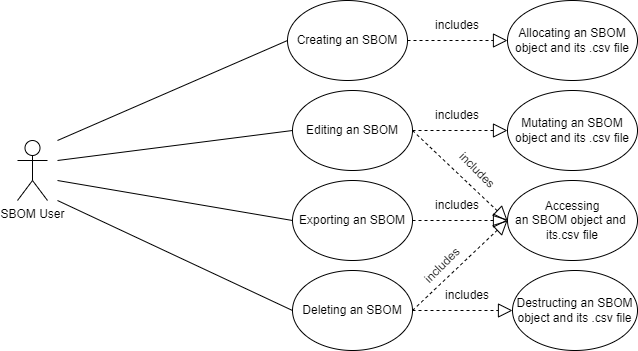
\includegraphics[width=1\linewidth]{SBOM_UseCase.drawio.png}
    \caption{SBOM Manager, Use Cases}
    \label{fig:enter-label}
\end{figure}
% use cases and usage scenarios - NOT OOP CLASSES

\section{Operating Environment}
\paragraph{ \normalfont
 Operating on a 64-bit system with Intel/AMD compatible architecture, running OpenBSD as the OS. Using the SQL database. Using iostream and fstream libraries. Being multi-user.
 \newline \newline
 Requiring 4GB of RAM and 10GB of disk space.
}

% client/server?
% multiuser?
% programming language?
% specific libraries or technology?
% CS server - OpenBSD, 64 bit, Intel/AMD compatible architecture,
% xx diskspace required?
% xx RAM required?
% ??? other ???

\section{Design and Implementation Constraints}
% restrictions on the software system design or implementation
\paragraph{ \normalfont
This project requires the usage of the C++ programming language, and the use of the web toolkit "Witty".
}

\chapter{NONFUNCTIONAL REQUIREMENTS}

\section{Performance Requirements}
\paragraph{ \normalfont
The system shall be capable of handling up to 50 simultaneous users without noticeable performance degradation. Each operation (create, edit, delete, export) should complete within 2 seconds under normal usage conditions.
}

\section{Safety Requirements}
\paragraph{ \normalfont
The software holds no risk of injury or death.
}

\section{Security Requirements}
\paragraph{ \normalfont
The application shall implement secure authentication using hashed passwords and ensure that all sensitive data is transmitted over encrypted channels (e.g., HTTPS). Only authorized users shall have access to their SBOMs, and the system shall implement user access controls to enforce this.
}

\section{Software Quality Attributes}
\subsection{Usability}
\paragraph{ \normalfont
The user interface shall achieve a usability score of 98 percent or higher in user satisfaction surveys, indicating that users can complete tasks without extensive training. The application shall provide feedback for successful and failed operations.
}

\subsection{Scalability}
\paragraph{ \normalfont
The system shall be designed to handle 200 users and SBOMs without significant changes to the codebase. % It should support at least 200 users as the project scales.
}

\subsection{Maintainability}
\paragraph{ \normalfont
The codebase shall be well-documented, with comments explaining complex logic. The design shall follow a modular architecture to allow for easy updates, bug fixes, and the addition of new features.
}

\subsection{Reliability and Availability}
\paragraph{ \normalfont
The system shall maintain an uptime of 99.9\%, meaning that it can experience no more than approximately 8.76 hours of downtime per year. The system shall be available 24/7, and any failures or crashes shall be logged for diagnostic purposes and shall not result in data corruption.
}

\subsection{Compatibility}
\paragraph{ \normalfont
The application shall be compatible with modern web browsers such as Chrome, Firefox, and Safari. Performance shall be measured by loading times of less than 3 seconds on supported browsers. It shall also run smoothly on the CS server's operating environment (OpenBSD on a 64-bit Intel/AMD compatible architecture).
}

\subsection{Data Integrity}
\paragraph{ \normalfont
The system shall ensure data consistency across all operations. Any data modifications (create, edit, delete) shall maintain the integrity of the SBOM entries and prevent accidental data corruption or loss. Data integrity shall be validated through regular audits, ensuring that no discrepancies exist in the SBOM entries.
}

\chapter{STANDARDS AND REFERENCES}
 
\section{Applicable Standards}

\subsection{ISO}
ISO/IEC 27001 A.9.4.2: Relates to ensuring systems use secure login mechanisms that protect a user's credentials during transmission, and preventing unauthorized access to the system.\\
ISO/IEC 27001 A.10.1: Ensures that a system is using the appropriate cyptographic measures to protect a user's sensitive data.

\subsection{IEEE}
IEEE SA Standards Board Operations Manual 6.4.7:  Lists guidelines for the usage and definition of the words 'shall', 'should', 'may', and 'can'.

% relevant standards, NIST? ISO? IEEE?

\section{References}
% list any documents cited in this document
\paragraph{ \normalfont
[1] G. Alvarenga, “What is an SBOM (software bill of materials)? - crowdstrike,” crowdstrike.com, https://www.crowdstrike.com/cybersecurity-101/secops/software-bill-of-materials-sbom/ (accessed Oct. 1, 2024). 
\newline \newline
[2] "Dependency-Track: Continuous SBOM Analysis Platform." OWASP, 2023. Accessed October 4, 2024. https://dependencytrack.org.
}

\end{document}
